\subsection{\large{\textit{cI}16-Si (Direct)}}\vspace{-0.1in}
Silicon (II)


\begin{figure}[H]
\begin{minipage}{0.34\textwidth}\centering
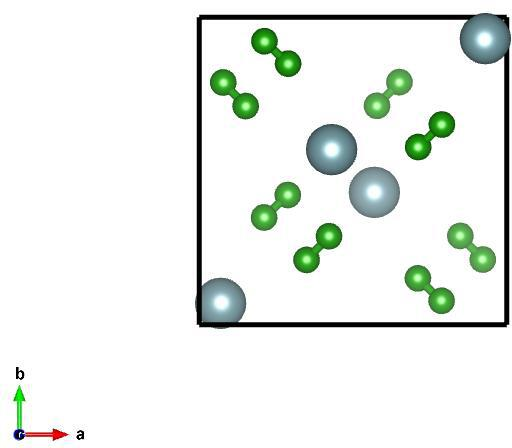
\includegraphics[width=0.9\linewidth,height=2in,keepaspectratio]{/Users/rosecers/work_folders/structures_for_photonics/reference/ref_inp/workspace/58abe2e5bb4b11d78f697ae66d2d7038/final_images/analog_trim.jpg}\\
\small{Image of \textit{cI}16-Si, generated by Vesta}
\end{minipage}\hfill
\begin{minipage}{0.65\textwidth}\raggedright
{\setlength{\mathindent}{0cm}
\begin{equation*}
\begin{split}&\boldsymbol{a_1} = -1/\sqrt{3}\ \hat{x} + 1/\sqrt{3}\ \hat{y} + 1/\sqrt{3}\ \hat{z}\\[-8pt]
&\boldsymbol{a_2} = 1/\sqrt{3}\ \hat{x} - 1/\sqrt{3}\ \hat{y} + 1/\sqrt{3}\ \hat{z}\\[-8pt]
&\boldsymbol{a_3} = 1/\sqrt{3}\ \hat{x} + 1/\sqrt{3}\ \hat{y} - 1/\sqrt{3}\ \hat{z}
\end{split}
\end{equation*}}

\textbf{Space Group:}	206\hspace{0.5in}\textbf{Point Group:}	$m\bar{3}$\\
\textbf{Inorganic Crystallographic Database} \#16569\\
\textbf{Structure DOI: }\url{10.1107/S0365110X64001840}

\end{minipage}\hfill
\end{figure}
\vspace{-0.25in}


\begin{figure}[H]
\begin{minipage}{0.9\textwidth}\centering
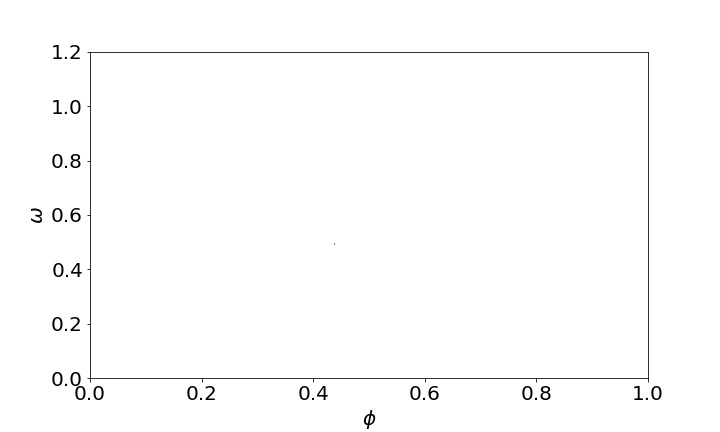
\includegraphics[width=0.9\linewidth,height=2.5in,keepaspectratio]{/Users/rosecers/work_folders/structures_for_photonics/reference/ref_inp/workspace/58abe2e5bb4b11d78f697ae66d2d7038/final_images/gap_atlas.jpg}
\\
\end{minipage}\hfill\caption{Gap Atlas across filling fraction $\phi$ and frequency $\omega$}
\end{figure}


\begin{figure}[H]
\begin{minipage}{0.5\textwidth}\centering
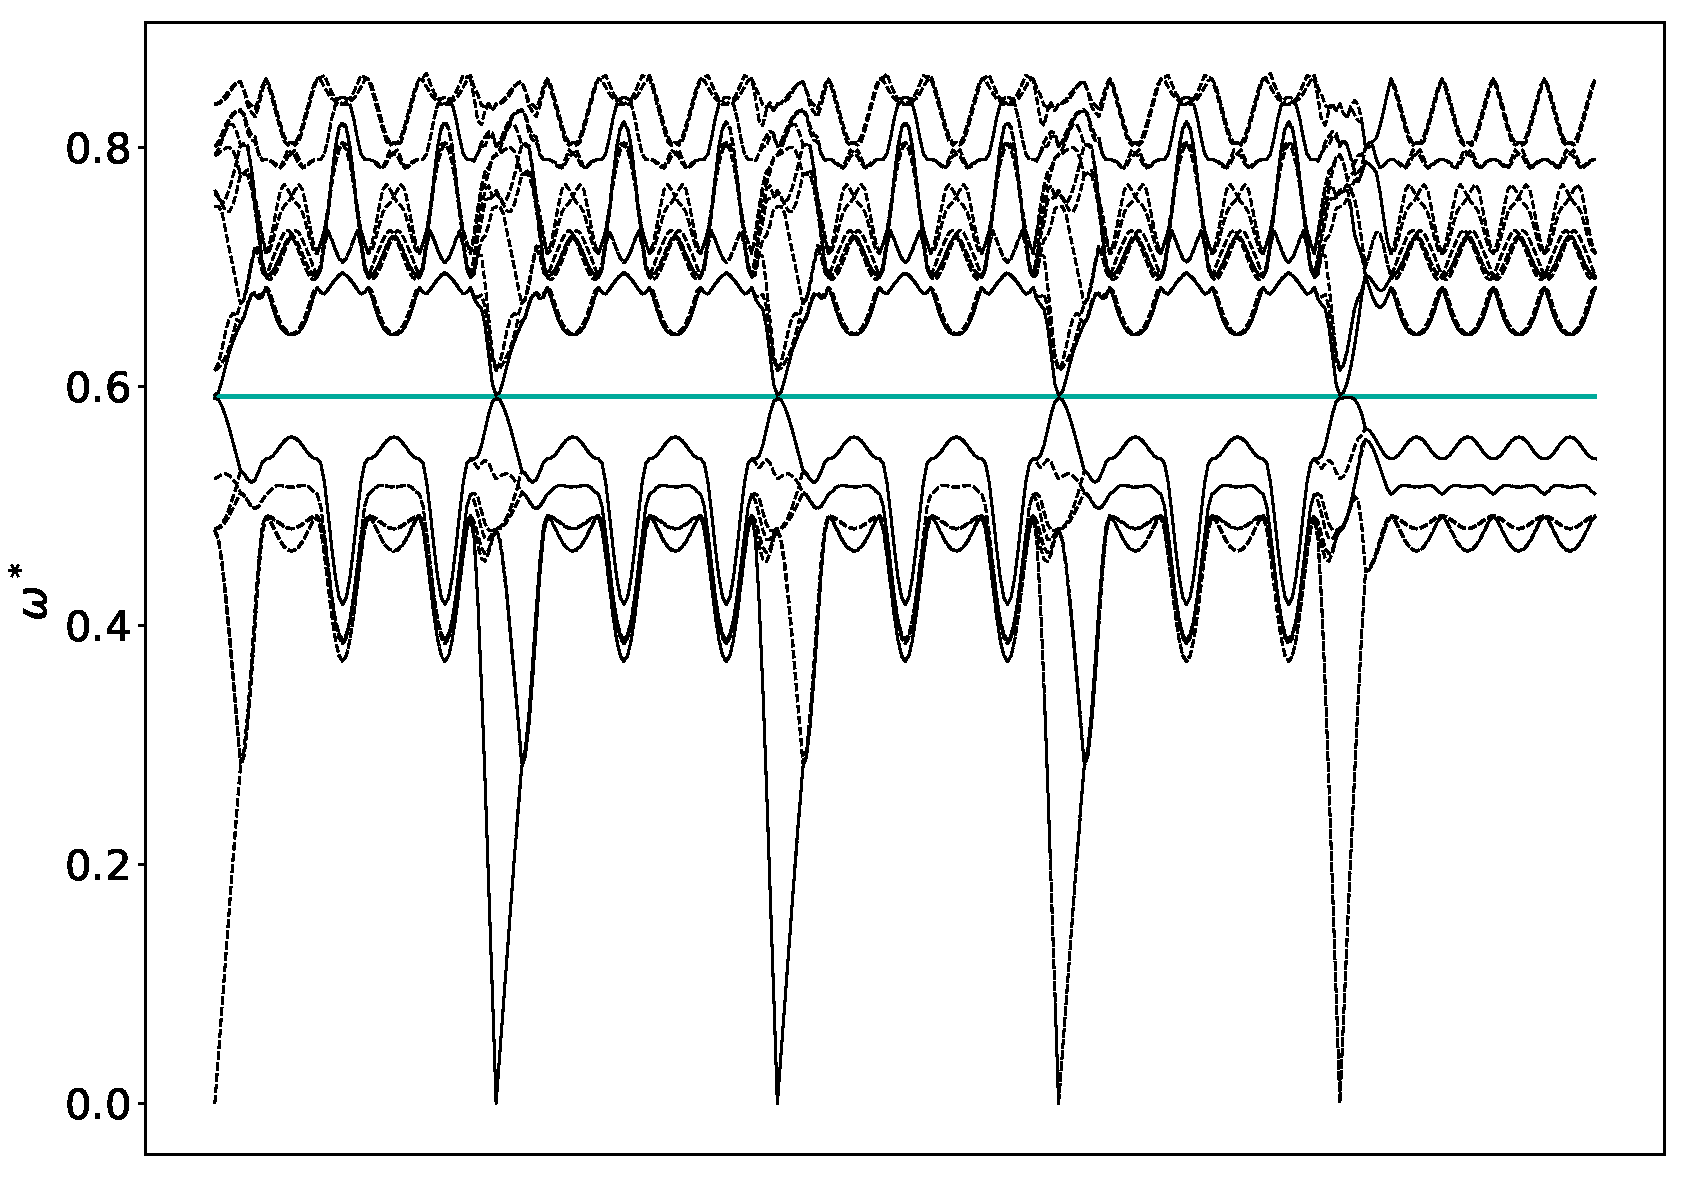
\includegraphics[width=0.9\linewidth,height=1.5in,keepaspectratio]{/Users/rosecers/work_folders/structures_for_photonics/reference/ref_inp/workspace/58abe2e5bb4b11d78f697ae66d2d7038/./final_images/band_diagram_b=8.pdf}
\\Band Structure across 1st BZ
\end{minipage}\hfill
\begin{minipage}{0.48\textwidth}\centering
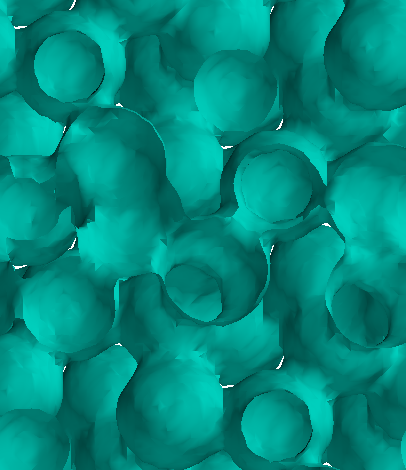
\includegraphics[width=0.9\linewidth,height=1.5in,keepaspectratio]{/Users/rosecers/work_folders/structures_for_photonics/reference/ref_inp/workspace/58abe2e5bb4b11d78f697ae66d2d7038/final_images/cI16-Si@gap_8-9.png}
\\View along $a_1$ 
\end{minipage}\hfill\caption{Band Structure and Isosurface of \textit{cI}16-Si (Direct) at radius = 0.225, filling fraction = 0.43, where the largest gap between bands 8 and 9 occurs with gap size 6.39\%.}

\end{figure}
\vspace{-0.25in}

